% Options for packages loaded elsewhere
% Options for packages loaded elsewhere
\PassOptionsToPackage{unicode}{hyperref}
\PassOptionsToPackage{hyphens}{url}
\PassOptionsToPackage{dvipsnames,svgnames,x11names}{xcolor}
%
\documentclass[
  letterpaper,
  DIV=11,
  numbers=noendperiod]{scrartcl}
\usepackage{xcolor}
\usepackage{amsmath,amssymb}
\setcounter{secnumdepth}{-\maxdimen} % remove section numbering
\usepackage{iftex}
\ifPDFTeX
  \usepackage[T1]{fontenc}
  \usepackage[utf8]{inputenc}
  \usepackage{textcomp} % provide euro and other symbols
\else % if luatex or xetex
  \usepackage{unicode-math} % this also loads fontspec
  \defaultfontfeatures{Scale=MatchLowercase}
  \defaultfontfeatures[\rmfamily]{Ligatures=TeX,Scale=1}
\fi
\usepackage{lmodern}
\ifPDFTeX\else
  % xetex/luatex font selection
\fi
% Use upquote if available, for straight quotes in verbatim environments
\IfFileExists{upquote.sty}{\usepackage{upquote}}{}
\IfFileExists{microtype.sty}{% use microtype if available
  \usepackage[]{microtype}
  \UseMicrotypeSet[protrusion]{basicmath} % disable protrusion for tt fonts
}{}
\makeatletter
\@ifundefined{KOMAClassName}{% if non-KOMA class
  \IfFileExists{parskip.sty}{%
    \usepackage{parskip}
  }{% else
    \setlength{\parindent}{0pt}
    \setlength{\parskip}{6pt plus 2pt minus 1pt}}
}{% if KOMA class
  \KOMAoptions{parskip=half}}
\makeatother
% Make \paragraph and \subparagraph free-standing
\makeatletter
\ifx\paragraph\undefined\else
  \let\oldparagraph\paragraph
  \renewcommand{\paragraph}{
    \@ifstar
      \xxxParagraphStar
      \xxxParagraphNoStar
  }
  \newcommand{\xxxParagraphStar}[1]{\oldparagraph*{#1}\mbox{}}
  \newcommand{\xxxParagraphNoStar}[1]{\oldparagraph{#1}\mbox{}}
\fi
\ifx\subparagraph\undefined\else
  \let\oldsubparagraph\subparagraph
  \renewcommand{\subparagraph}{
    \@ifstar
      \xxxSubParagraphStar
      \xxxSubParagraphNoStar
  }
  \newcommand{\xxxSubParagraphStar}[1]{\oldsubparagraph*{#1}\mbox{}}
  \newcommand{\xxxSubParagraphNoStar}[1]{\oldsubparagraph{#1}\mbox{}}
\fi
\makeatother


\usepackage{longtable,booktabs,array}
\usepackage{calc} % for calculating minipage widths
% Correct order of tables after \paragraph or \subparagraph
\usepackage{etoolbox}
\makeatletter
\patchcmd\longtable{\par}{\if@noskipsec\mbox{}\fi\par}{}{}
\makeatother
% Allow footnotes in longtable head/foot
\IfFileExists{footnotehyper.sty}{\usepackage{footnotehyper}}{\usepackage{footnote}}
\makesavenoteenv{longtable}
\usepackage{graphicx}
\makeatletter
\newsavebox\pandoc@box
\newcommand*\pandocbounded[1]{% scales image to fit in text height/width
  \sbox\pandoc@box{#1}%
  \Gscale@div\@tempa{\textheight}{\dimexpr\ht\pandoc@box+\dp\pandoc@box\relax}%
  \Gscale@div\@tempb{\linewidth}{\wd\pandoc@box}%
  \ifdim\@tempb\p@<\@tempa\p@\let\@tempa\@tempb\fi% select the smaller of both
  \ifdim\@tempa\p@<\p@\scalebox{\@tempa}{\usebox\pandoc@box}%
  \else\usebox{\pandoc@box}%
  \fi%
}
% Set default figure placement to htbp
\def\fps@figure{htbp}
\makeatother


% definitions for citeproc citations
\NewDocumentCommand\citeproctext{}{}
\NewDocumentCommand\citeproc{mm}{%
  \begingroup\def\citeproctext{#2}\cite{#1}\endgroup}
\makeatletter
 % allow citations to break across lines
 \let\@cite@ofmt\@firstofone
 % avoid brackets around text for \cite:
 \def\@biblabel#1{}
 \def\@cite#1#2{{#1\if@tempswa , #2\fi}}
\makeatother
\newlength{\cslhangindent}
\setlength{\cslhangindent}{1.5em}
\newlength{\csllabelwidth}
\setlength{\csllabelwidth}{3em}
\newenvironment{CSLReferences}[2] % #1 hanging-indent, #2 entry-spacing
 {\begin{list}{}{%
  \setlength{\itemindent}{0pt}
  \setlength{\leftmargin}{0pt}
  \setlength{\parsep}{0pt}
  % turn on hanging indent if param 1 is 1
  \ifodd #1
   \setlength{\leftmargin}{\cslhangindent}
   \setlength{\itemindent}{-1\cslhangindent}
  \fi
  % set entry spacing
  \setlength{\itemsep}{#2\baselineskip}}}
 {\end{list}}
\usepackage{calc}
\newcommand{\CSLBlock}[1]{\hfill\break\parbox[t]{\linewidth}{\strut\ignorespaces#1\strut}}
\newcommand{\CSLLeftMargin}[1]{\parbox[t]{\csllabelwidth}{\strut#1\strut}}
\newcommand{\CSLRightInline}[1]{\parbox[t]{\linewidth - \csllabelwidth}{\strut#1\strut}}
\newcommand{\CSLIndent}[1]{\hspace{\cslhangindent}#1}



\setlength{\emergencystretch}{3em} % prevent overfull lines

\providecommand{\tightlist}{%
  \setlength{\itemsep}{0pt}\setlength{\parskip}{0pt}}



 


\KOMAoption{captions}{tableheading}
\makeatletter
\@ifpackageloaded{caption}{}{\usepackage{caption}}
\AtBeginDocument{%
\ifdefined\contentsname
  \renewcommand*\contentsname{Table of contents}
\else
  \newcommand\contentsname{Table of contents}
\fi
\ifdefined\listfigurename
  \renewcommand*\listfigurename{List of Figures}
\else
  \newcommand\listfigurename{List of Figures}
\fi
\ifdefined\listtablename
  \renewcommand*\listtablename{List of Tables}
\else
  \newcommand\listtablename{List of Tables}
\fi
\ifdefined\figurename
  \renewcommand*\figurename{Figure}
\else
  \newcommand\figurename{Figure}
\fi
\ifdefined\tablename
  \renewcommand*\tablename{Table}
\else
  \newcommand\tablename{Table}
\fi
}
\@ifpackageloaded{float}{}{\usepackage{float}}
\floatstyle{ruled}
\@ifundefined{c@chapter}{\newfloat{codelisting}{h}{lop}}{\newfloat{codelisting}{h}{lop}[chapter]}
\floatname{codelisting}{Listing}
\newcommand*\listoflistings{\listof{codelisting}{List of Listings}}
\makeatother
\makeatletter
\makeatother
\makeatletter
\@ifpackageloaded{caption}{}{\usepackage{caption}}
\@ifpackageloaded{subcaption}{}{\usepackage{subcaption}}
\makeatother
\usepackage{bookmark}
\IfFileExists{xurl.sty}{\usepackage{xurl}}{} % add URL line breaks if available
\urlstyle{same}
\hypersetup{
  pdftitle={Why adding uncertainty into regional GVA is a good thing},
  pdfauthor={Dan Olner},
  colorlinks=true,
  linkcolor={blue},
  filecolor={Maroon},
  citecolor={Blue},
  urlcolor={Blue},
  pdfcreator={LaTeX via pandoc}}


\title{Why adding uncertainty into regional GVA is a good thing}
\author{Dan Olner}
\date{2026-02-11}
\begin{document}
\maketitle

\renewcommand*\contentsname{Table of contents}
{
\hypersetup{linkcolor=}
\setcounter{tocdepth}{3}
\tableofcontents
}

\subsection{Things to stick in}\label{things-to-stick-in}

\begin{itemize}
\tightlist
\item
  Make clear this is focused on thinking through regional econ strategy
  and what difference it makes for that specifically.
\end{itemize}

\subsection{Headlines}\label{headlines}

\begin{itemize}
\item
\item
  This is in large part due to the constrictions of the (globally agreed
  so extremely slow to change) System of National Accounts (Coyle 2014).
\item
  Far from just introducing less precision, including uncertainty leads
  to some quite different, useful ways of thinking about regions,
  grounded in what we do and don't know.
\item
  I might argue - it's more powerful, because it short-circuits many
  unhelpful ways of thinking about growth and industrial strategy (some
  built right into the foundation e.g.~see the CIA Russia assessment).
\end{itemize}

\subsection{Resources/links}\label{resourceslinks}

I have prepared two interactive web pages for each of the GVA sources
discussed below. I'll refer back to these with links.

\begin{enumerate}
\def\labelenumi{\arabic{enumi}.}
\item
  \href{https://danolner.github.io/RegEconWorks/growth_errorgrids_viewer/}{Chained
  volume GVA}: What is the growth signal if error rates are included in
  regional data?
\item
  \href{https://danolner.github.io/RegEconWorks/lq-errorbars-viewer/}{Current
  prices GVA}: What happens to location quotients if error rates are
  included?
\end{enumerate}

\subsection{Introduction: how to avoid chasing vampires off cliff
edges}\label{introduction-how-to-avoid-chasing-vampires-off-cliff-edges}

In the movie `The Lost Boys', David and his west-coast vampire buddies
\href{https://youtu.be/DP_lSpeK69c?si=klxDzst0hVvV0QlY}{race motorbikes
across a misty landscape}. Michael (as yet unaware of the blood-drinking
habits of his new associates) tries to keep up with them. They egg him
on - but then he spots the faint beam of a lighthouse, puts two and two
together and barely avoids hurtling over a cliff edge.

One might say David was claiming `incredible certitude' (Manski 2020)
about the cliff's location. ``Don't worry Micheal, it's definitely,
definitely miles from here.''

If there's fog, what you do about that depends on what you think is
going on / what else you feel certain about. But the fog matters, the
fog itself is information. (i.e.~fog near a cliff is different info to
fog walking on an open moor).

\subsection{Being constructive in a noisy
argument}\label{being-constructive-in-a-noisy-argument}

Put this in resources as its own thing/post. Would allow discussion of
`concern trolling' a bit?

\subsection{Getting away from perfect
sums}\label{getting-away-from-perfect-sums}

The issues all stem from the same root: national accounts methods (1)
are designed to analyse nations, not regions, and (2) are accounts. They
have to balance, every part of the economy has to add up correctly and
consistently - including across all UK regions. This forces a
national-level, top-down straitjacket on regional numbers. Let's make a
start in this post on one of the most important consequences of that:

\begin{itemize}
\tightlist
\item
  Accounts only report single values. It's all they \emph{can} report.
  Uncertainty doesn't feature.
\end{itemize}

Through this lens, the UK
\href{https://www.ons.gov.uk/economy/grossdomesticproductgdp/bulletins/gdpmonthlyestimateuk/november2025}{grew
by exactly} 0.1\% in the three months to November 2025. Uncertainty only
enters via later revisions to those exact figures - the image here is
\href{https://www.ons.gov.uk/economy/grossdomesticproductgdp/articles/communicatinggrossdomesticproduct/2020-04-16}{from
the ONS} showing how much revisions over time differ from initial
numbers. These are very much \emph{not} confidence intervals showing the
underlying uncertainty in the data.

And they try to do this work when
\href{https://www.bbc.co.uk/news/articles/cwyp7v7r28yo}{chancellors and
shadow chancellors shout and point fingers} over every 0.1\% revision.
Argh.

Or: the ONS have no choice here - the national accounts
straitjacket\ldots{}

In the
\href{https://www.ons.gov.uk/economy/grossvalueaddedgva/methodologies/regionalgrossvalueaddedbalancedqmi}{ONS'
method doc} for regional GVA, they explicitly say:

\begin{quote}
``The complex process by which GVA estimates are produced means that it
is not currently possible to define the accuracy of the
estimates\ldots{} for example, through their standard errors. Therefore,
the reliability of the estimates is measured by the extent of
revisions.''
\end{quote}

I think ONS are doing themselves a disservice here - they could
certainly handle the complexity. It's just the `accounting' point again:
the assembly of national output involves so many moving parts, and the
need for perfect
\href{https://www.ons.gov.uk/economy/grossdomesticproductgdp/articles/recentchallengesofbalancingthethreeapproachesofgdp/2022-04-20}{balancing}
(however baroque) so built-in, there just isn't scope to do anything
else with regional economic numbers.

The uncertainty, however, hasn't gone away. In this post, I'll have a go
at showing what difference the uncertainty could make to the numbers, if
we could see it.

That's a different (though of course linked) question from ``If things
are uncertain, how does that change how we should act?'' I'll come to
that one in a later post (I'm just reading Manski's
\href{https://www.cambridge.org/core/journals/economics-and-philosophy/article/abs/lure-of-incredible-certitude/A1F09783377B05F20B83543CD40C7639}{Lure
of Incredible Certitude} to warm up for that).

This is all a slightly alarming look back at the certitude I've built
into my own work too. It's very difficult to resist, both methods-wise
(single values is all we have, often) and
what-policymakers-want-to-see-wise. One of my plots below
(\href{https://danolner.github.io/RegionalEconomicTools/gdp_gaps.html}{code
here}) is a prime example: GVA per hour, ITL2 zones ranked! Who's up,
who's down on the scoreboard??

\subsection{Making a data-driven guess about the level of regional GVA
uncertainty}\label{making-a-data-driven-guess-about-the-level-of-regional-gva-uncertainty}

The \textbf{Annual Business Survey (ABS)} is a good source that allows
an educated guess of confidence bounds around regional/sectoral GVA
data. It is
\href{https://www.ons.gov.uk/businessindustryandtrade/business/businessservices/methodologies/annualbusinesssurveyqmi}{designed}
to capture sectoral and regional GVA at a reasonable resolution. As the
ONS
\href{https://www.ons.gov.uk/economy/grossvalueaddedgva/articles/analysisoftheextentofmodellingandestimationinregionalgrossvalueadded/2018-03-28\#principal-data-sources-used-in-regional-gross-value-added}{say}
in their fascinating breakdown (if you're into that kind of thing) of
``observed/estimated/modelled components of regional GVA'':

\begin{quote}
Of all the data sources used in regional GVA, the ABS has the greatest
overall impact, representing around 71\% of GVA(P) and 22\% of
GVA(I)\ldots{} It includes elements corresponding to all three of the
categories of data we wish to analyse: directly collected from
businesses operating in a single region; weighted to represent
non-sampled businesses; and apportioned to regions from UK-wide company
information.
\end{quote}

Data comes direct from firms- there is much less reliance on some of the
more
\href{https://exobrain.coveredinbees.org/attachments/heroic-assumptions/}{heroic
assumptions} that go into other aspects of regional GVA. {[}Roadmap:
exploring the implications of assumptions for finance, telecoms and
public sectors{]}.

The publically available ABS sources are broken into the
\href{https://www.ons.gov.uk/businessindustryandtrade/business/businessservices/datasets/uknonfinancialbusinesseconomyannualbusinesssurveyregionalresultssectionsas}{central
estimate data} and
\href{https://www.ons.gov.uk/businessindustryandtrade/business/businessservices/datasets/uknonfinancialbusinesseconomyannualbusinesssurveyregionalresultsqualitymeasures}{error
data}\footnote{\href{https://github.com/DanOlner/RegionalEconomicTools/blob/gh-pages/bits_of_code/ABS_error_rates.R}{code/comments
  here} run through combining those two sources. A final joined CSV is
  \href{https://github.com/DanOlner/RegionalEconomicTools/blob/gh-pages/data/abs_gva_se_combo.csv}{here},
  to save others the pain, though it's just for GVA, not every ABS
  value.} giving GVA values and standard errors at ITL1 geography level
and 2-digit SIC sectors. Here, I convert GVA and standard errors from
the ABS to coefficients of variation (proportion of error) and then
apply them to the regional/sectoral GVA national accounts data at the
same geogaphical scale, and where sectors are present in both sources
(there are 73 that match once ABS sector categories are processed to
match the region/sector data's bespoke SIC list). Only years available
in both sources are used - 2012 to 2023.

Below, I'll explore the implications of these error rates when applied
both available types of GVA data:

\begin{itemize}
\tightlist
\item
  Chained volume (CV) data that aims to capture `real' output changes
  over time. From these, we can ask, ``Did this sector grow or shrink
  here?'' We can do a few other things e.g.~was its growth slope really
  steeper than other places?
\item
  Current prices (CP) data, which (being prices as they were in the year
  they were counted) can be summed, and used to look at location
  quotients (LQs) - how concentrated a sector is in each place. It's
  where we can get a good sense of the UK's economic structure, because
  it's possible to compare sizes across the UK. We'll have a go at
  adding error rates to LQs.
\end{itemize}

For both of those, the question is: ``If the regional GVA data had the
same error rates as the ABS, what would it look like and what would some
implications for analysis be?''

Are those reasonable questions to ask? Two points.

\begin{enumerate}
\def\labelenumi{\arabic{enumi}.}
\item
  This is testing an ``if then.'' If the error rates were this,
  then\ldots{} For those sectors that match, I think it's a fair
  assumption that the ABS reasonably captures its uncertainty. Adding
  extra sources would be unlikely to reduce it much.
\item
  The alternative is working with the point data as if it was perfectly
  accurate. Seeing what difference error makes - even if there's error
  in our error - leads to quite different ways of thinking.
\end{enumerate}

\subsection{Chained volume data}\label{chained-volume-data}

Chained volume data is used to assess real economic change over time,
accounting for inflation and quality changes in goods. Change in CV
values over time should represent actual growth or shrinkage in a
particular sector and place. This section limits itself to asking how
much the growth signal changes for individual sectors in specific ITL1s
with the inclusion of error rates.

{[}It doesn't use those errors to compare sectors across places\ldots{}
though might do this quickly\ldots{} simulation again to add to CAGR{]}

The
\href{https://danolner.github.io/RegEconWorks/growth_errorgrids_viewer/}{interactive
here} provides a way to look at individual sectors across all twelve
ITL1 zones.

\begin{itemize}
\item
  The inclusion of error rates immediately makes it very rare for
  year-to-year changes to be distinguishable from zero. So instead, what
  each grid plot does is compare each year to every other year, to show
  where each is clearly separable.
\item
  The assumptions used (on top of the if/then above) are: 95\%
  confidence intervals, and assuming that change isn't definitely
  present if the minimum from one year is lower than the maximum from
  another year (and vice versa). This is a conservative assumption that
  the true value\footnote{`True value' being used as shorthand for the
    cumbersome `95\% confidence interval would contain the true value
    95\% of the time if the survey sample was taken again'. {[}ONS
    source\ldots{]}} could be at both confidence extremes between
  timepoints.
\end{itemize}

Let's talk through the default sector, fabricated metals, to make more
sense of that. Consider the example in Figure~\ref{fig-ynhfab} - in the
interactive, hover over Yorkshire and Humber to see its growth over
time. What this shows:

\begin{itemize}
\item
  Blue squares in the grid indicate that the column year was clearly
  higher than the row year it is compared to (`clearly' as described
  above).
\item
  We can see that 2020 to 2023 are clearly higher than the earlier years
  in the data, from 2012 to 2016, though the high peak in 2021 is the
  only year consistently separable from others. 2020 to 2023 are years
  where the confidence interval minimum is separable from the earlier CI
  maxima.
\item
  The rest of the grey area is showing that, for the first half of the
  data from 2012 to 2017 - on the assumptions we have here - no clear
  growth signal is coming through.
\item
  Note, the grid is mirrored along the diagonal: here, orange squares
  are showing the same thing in reverse - earlier column years are
  clearly lower than some later ones.
\end{itemize}

\begin{figure}

\centering{

\pandocbounded{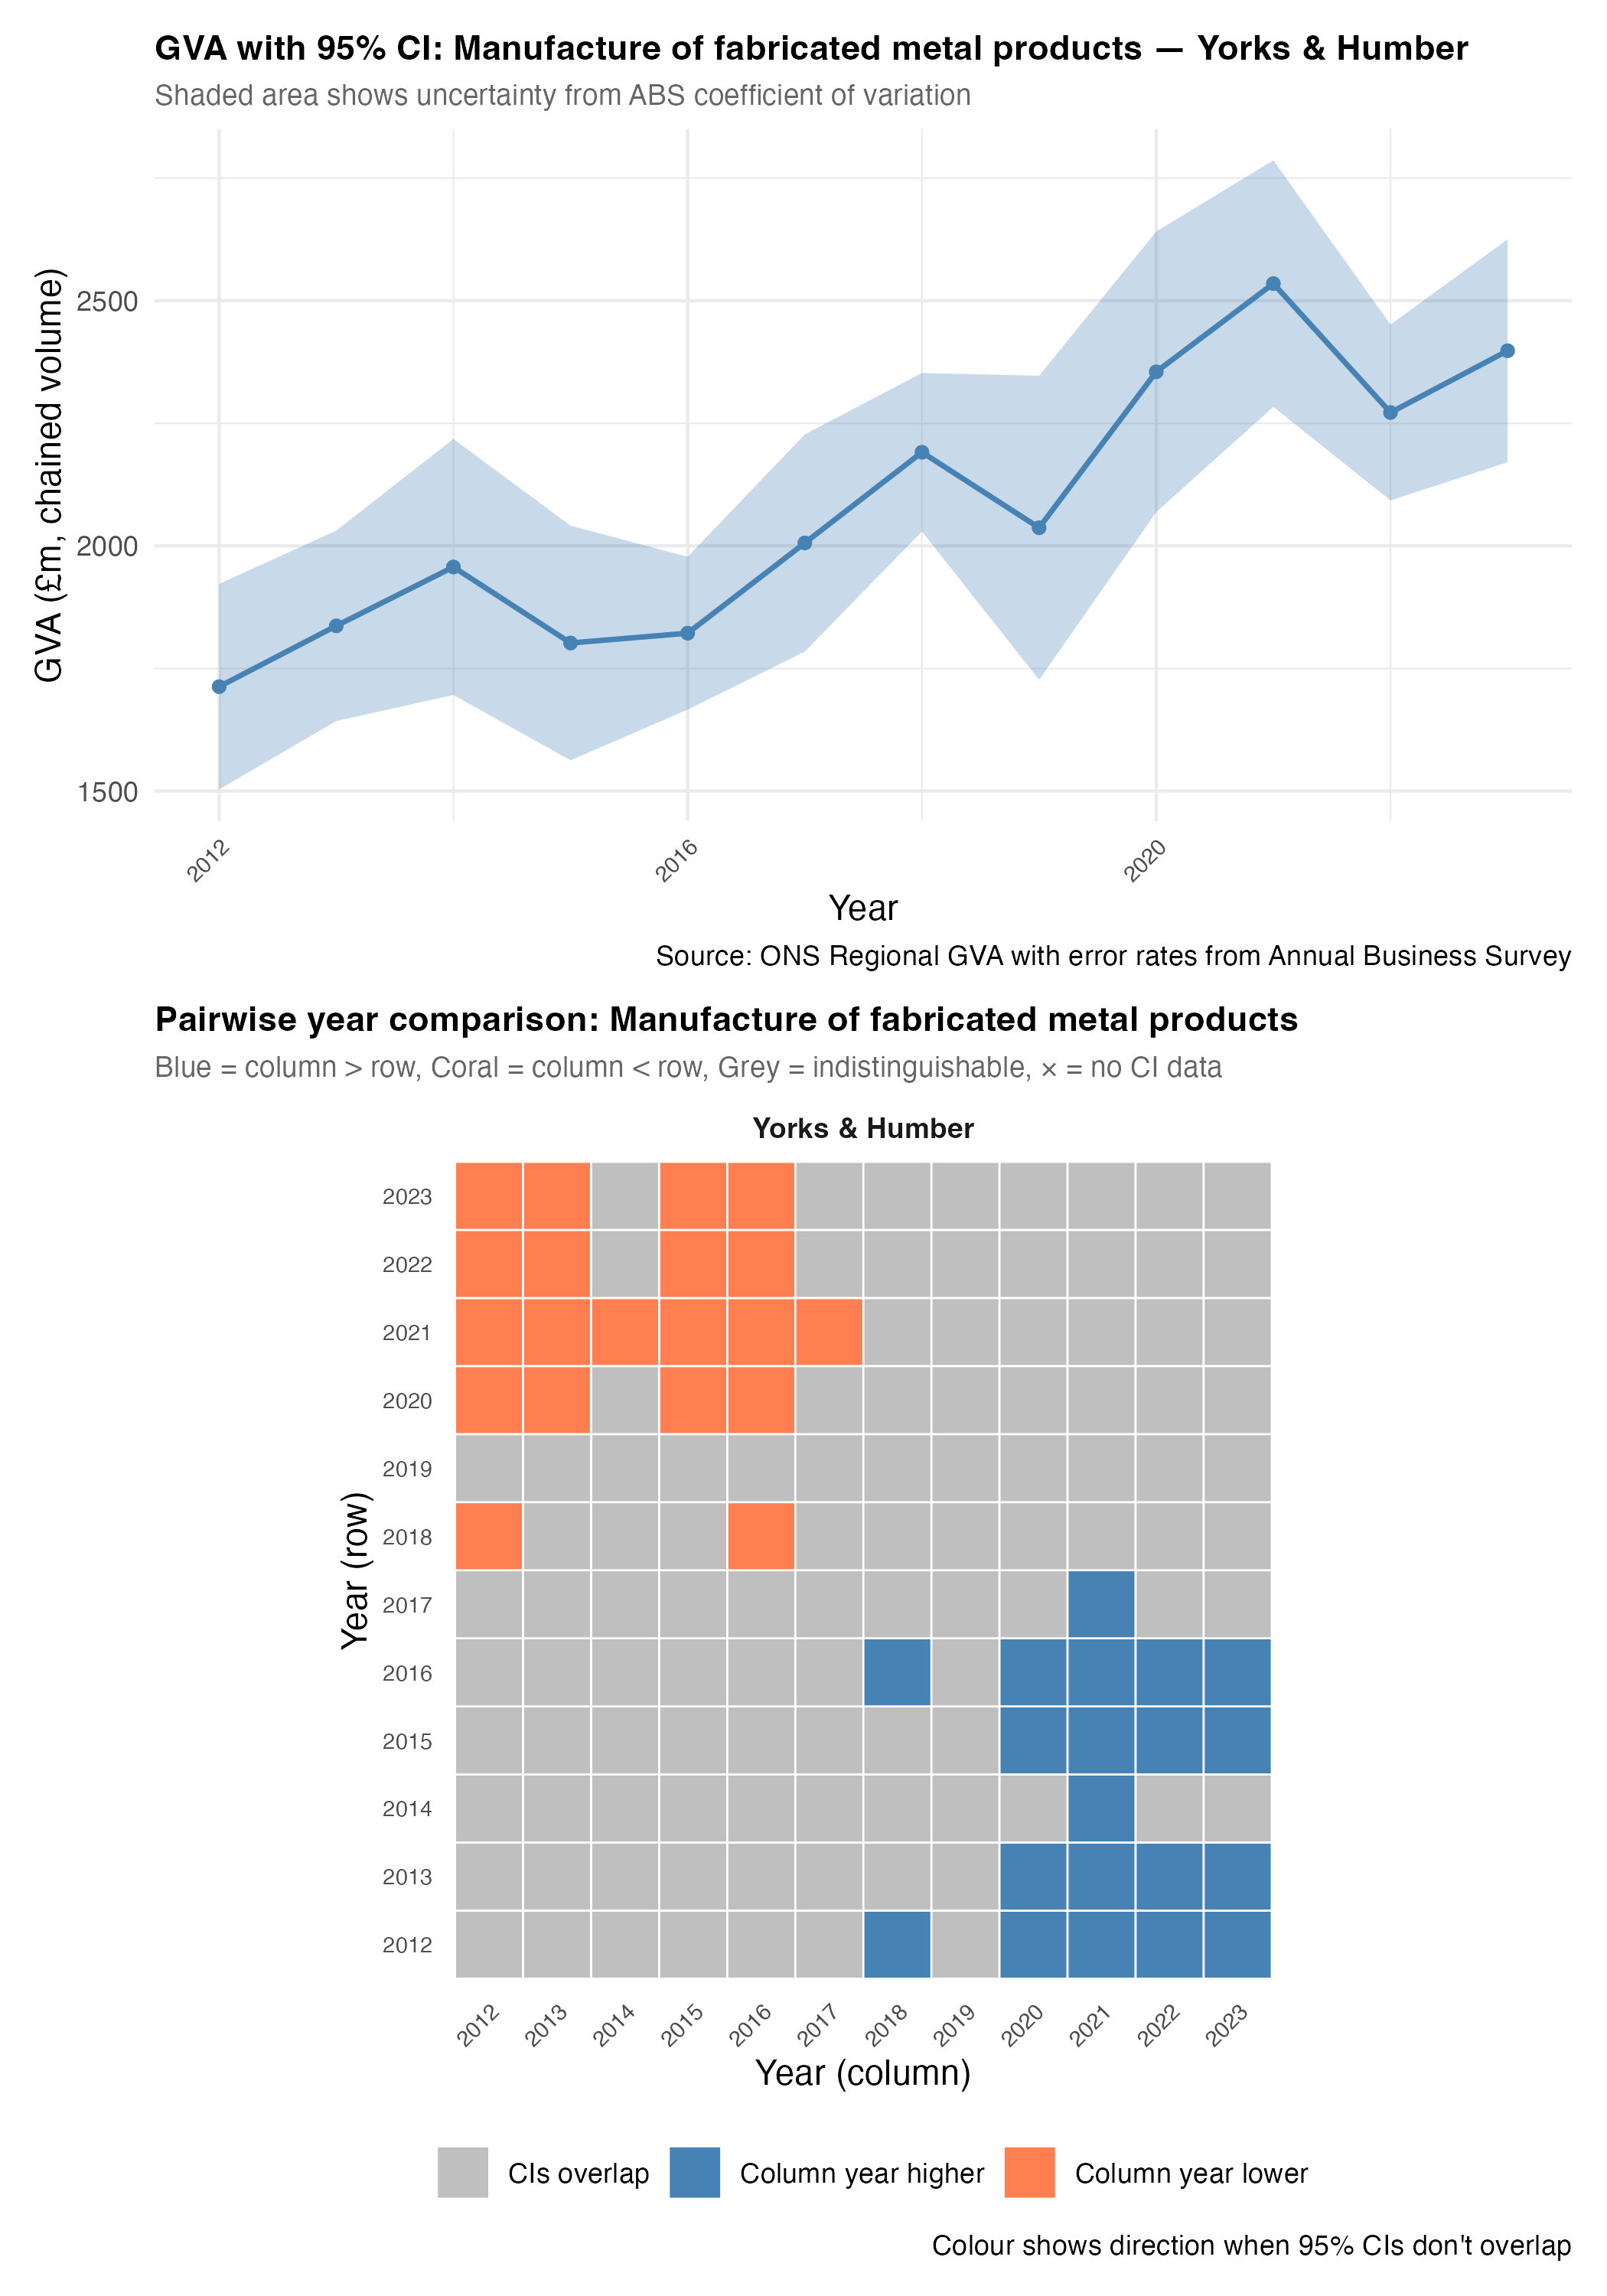
\includegraphics[keepaspectratio]{images/YNH_growthgrid.png}}

}

\caption{\label{fig-ynhfab}Yorkshire \& Humber GVA growth grid and
growth over time, fabricated metals.}

\end{figure}%

Scotland shows the opposite pattern, which can be seen from its growth
slope clearly too - bottom left orange squares indicate clearly lower
values in the later part of the data. Figure~\ref{fig-eastmidsfab} is
showing that, while the later value increases appear separable from the
low point around 2017, it can't be so easily distinguished from where it
was from 2012 to 2016. Several other ITLs are purely grey. Looking at
any of those shows combinations of wide error rates and fairly flat
change over time, considering the range of those confidence intervals.
The apparent drop in the North West after 2017, for example, isn't
clearly separable, though it looks strong. Other sources could help
support or question that apparent change.

\begin{figure}

\centering{

\pandocbounded{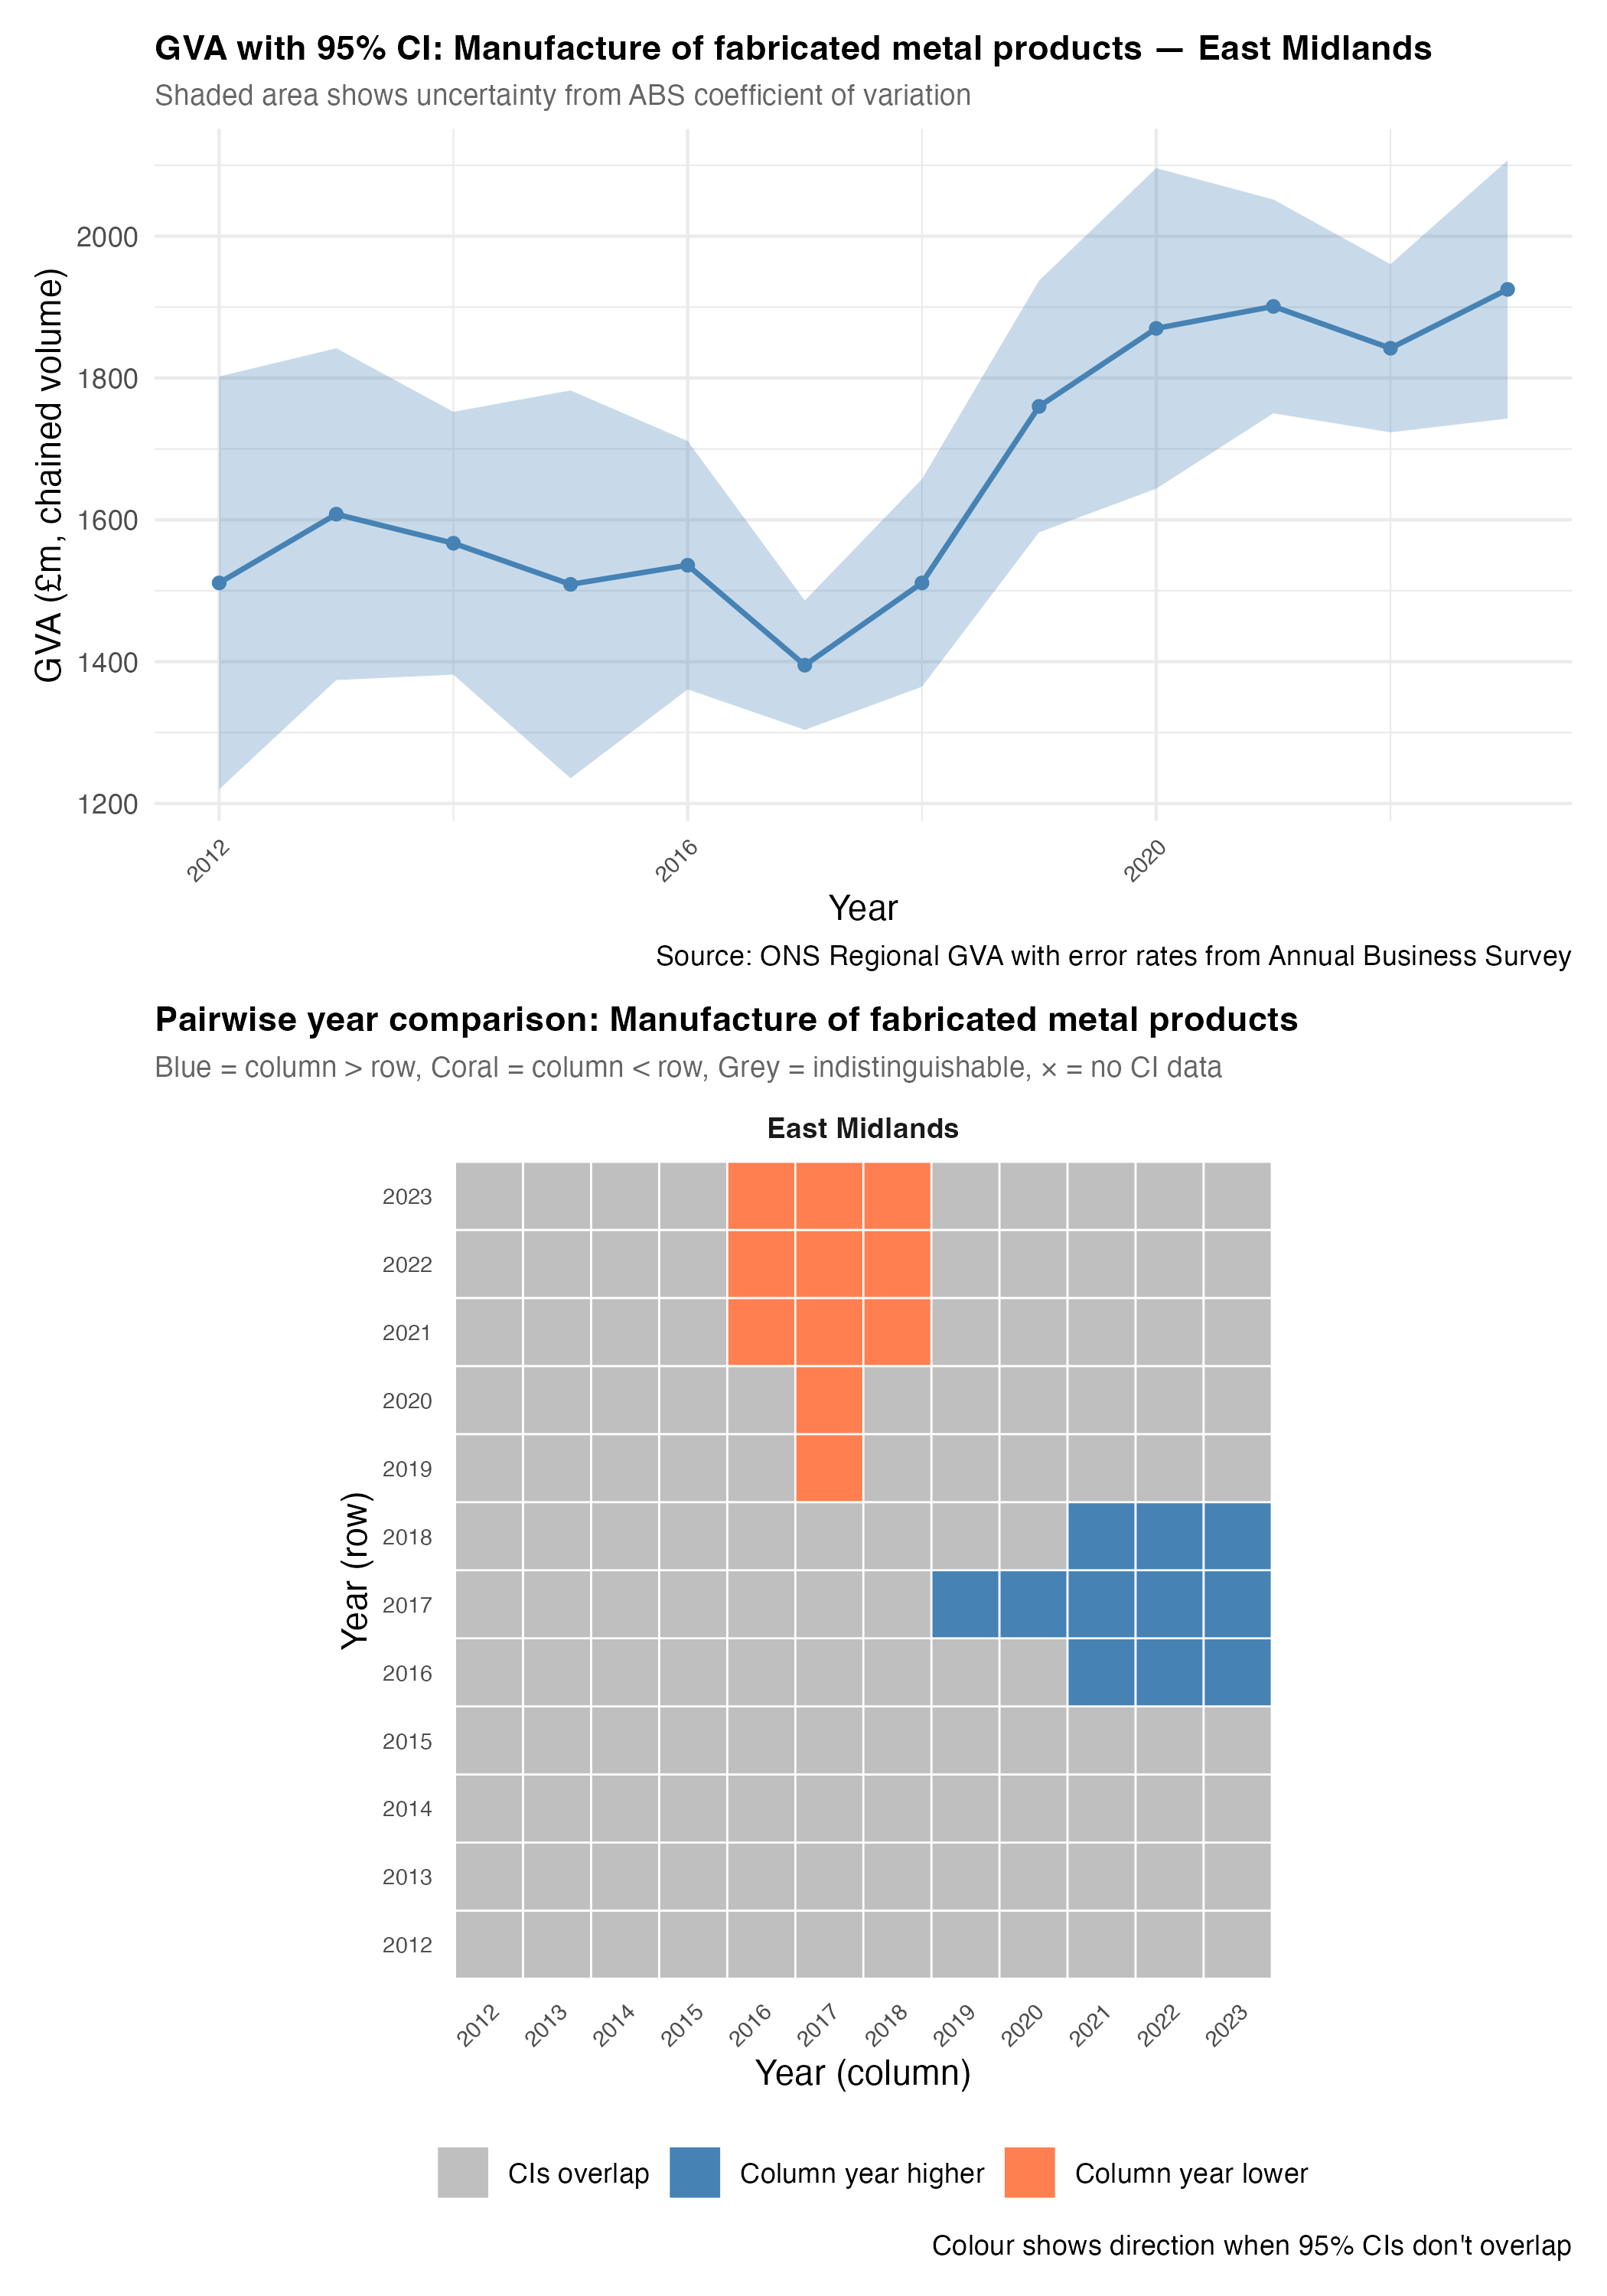
\includegraphics[keepaspectratio]{images/eastmids_growthgrid.png}}

}

\caption{\label{fig-eastmidsfab}East Midlands GVA growth grid and growth
over time, fabricated metals}

\end{figure}%

Other notable patterns are discussed in a section at the end of this
document.

The binary cutoffs here are stark - this is a common issue with
threshold-based statistical approaches\ldots{} discuss pros and cons and
say still probably better than the alternative. Consider these as part
of decision-making under uncertainty. What does that look like?

\phantomsection\label{refs}
\begin{CSLReferences}{1}{0}
\bibitem[\citeproctext]{ref-coyle2014}
Coyle, Diane. 2014. \emph{GDP: A Brief but Affectionate History}.
Princeton University Press.

\bibitem[\citeproctext]{ref-manski2020}
Manski, Charles F. 2020. {``The lure of incredible certitude.''}
\emph{Economics and philosophy} 36 (2): 216245.
\url{https://doi.org/10.1017/S0266267119000105}.

\end{CSLReferences}




\end{document}
